\documentclass[a4paper,12pt,twoside]{memoir}

% Castellano
\usepackage[spanish,es-tabla]{babel}
\selectlanguage{spanish}
\usepackage[utf8]{inputenc}
\usepackage[T1]{fontenc}
\usepackage{lmodern} % scalable font
\usepackage{microtype}
\usepackage{placeins}
\usepackage{eurosym}
\RequirePackage{booktabs}
\RequirePackage[table]{xcolor}
\RequirePackage{xtab}
\RequirePackage{multirow}
\usepackage[linesnumbered,ruled,spanish,onelanguage]{algorithm2e}
% Links
\usepackage[colorlinks]{hyperref}
\hypersetup{
	allcolors = {red}
}

% Ecuaciones
\usepackage{amsmath}

% Rutas de fichero / paquete
\newcommand{\ruta}[1]{{\sffamily #1}}

% Párrafos
\nonzeroparskip


% Imagenes
\usepackage{graphicx}
\newcommand{\imagen}[2]{
	\begin{figure}[!h]
		\centering
		\includegraphics[width=0.9\textwidth]{#1}
		\caption{#2}\label{fig:#1}
	\end{figure}
	\FloatBarrier
}

\newcommand{\imagenflotante}[2]{
	\begin{figure}%[!h]
		\centering
		\includegraphics[width=0.9\textwidth]{#1}
		\caption{#2}\label{fig:#1}
	\end{figure}
}



% El comando \figura nos permite insertar figuras comodamente, y utilizando
% siempre el mismo formato. Los parametros son:
% 1 -> Porcentaje del ancho de página que ocupará la figura (de 0 a 1)
% 2 --> Fichero de la imagen
% 3 --> Texto a pie de imagen
% 4 --> Etiqueta (label) para referencias
% 5 --> Opciones que queramos pasarle al \includegraphics
% 6 --> Opciones de posicionamiento a pasarle a \begin{figure}
\newcommand{\figuraConPosicion}[6]{%
	\setlength{\anchoFloat}{#1\textwidth}%
	\addtolength{\anchoFloat}{-4\fboxsep}%
	\setlength{\anchoFigura}{\anchoFloat}%
	\begin{figure}[#6]
		\begin{center}%
			\Ovalbox{%
				\begin{minipage}{\anchoFloat}%
					\begin{center}%
						\includegraphics[width=\anchoFigura,#5]{#2}%
						\caption{#3}%
						\label{#4}%
					\end{center}%
				\end{minipage}
			}%
		\end{center}%
	\end{figure}%
}

%
% Comando para incluir imágenes en formato apaisado (sin marco).
\newcommand{\figuraApaisadaSinMarco}[5]{%
	\begin{figure}%
		\begin{center}%
			\includegraphics[angle=90,height=#1\textheight,#5]{#2}%
			\caption{#3}%
			\label{#4}%
		\end{center}%
	\end{figure}%
}
% Para las tablas
\newcommand{\otoprule}{\midrule [\heavyrulewidth]}
%
% Nuevo comando para tablas pequeñas (menos de una página).
\newcommand{\tablaSmall}[5]{%
	\begin{table}
		\begin{center}
			\rowcolors {2}{gray!35}{}
			\begin{tabular}{#2}
				\toprule
				#4
				\otoprule
				#5
				\bottomrule
			\end{tabular}
			\caption{#1}
			\label{tabla:#3}
		\end{center}
	\end{table}
}

%
%Para el float H de tablaSmallSinColores
\usepackage{float}

%
% Nuevo comando para tablas pequeñas (menos de una página).
\newcommand{\tablaSmallSinColores}[5]{%
	\begin{table}[H]
		\begin{center}
			\begin{tabular}{#2}
				\toprule
				#4
				\otoprule
				#5
				\bottomrule
			\end{tabular}
			\caption{#1}
			\label{tabla:#3}
		\end{center}
	\end{table}
}

\newcommand{\tablaApaisadaSmall}[5]{%
	\begin{landscape}
		\begin{table}
			\begin{center}
				\rowcolors {2}{gray!35}{}
				\begin{tabular}{#2}
					\toprule
					#4
					\otoprule
					#5
					\bottomrule
				\end{tabular}
				\caption{#1}
				\label{tabla:#3}
			\end{center}
		\end{table}
	\end{landscape}
}

%
% Nuevo comando para tablas grandes con cabecera y filas alternas coloreadas en gris.
\newcommand{\tabla}[6]{%
	\begin{center}
		\tablefirsthead{
			\toprule
			#5
			\otoprule
		}
		\tablehead{
			\multicolumn{#3}{l}{\small\sl continúa desde la página anterior}\\
			\toprule
			#5
			\otoprule
		}
		\tabletail{
			\hline
			\multicolumn{#3}{r}{\small\sl continúa en la página siguiente}\\
		}
		\tablelasttail{
			\hline
		}
		\bottomcaption{#1}
		\rowcolors {2}{gray!35}{}
		\begin{xtabular}{#2}
			#6
			\bottomrule
		\end{xtabular}
		\label{tabla:#4}
	\end{center}
}

%
% Nuevo comando para tablas grandes con cabecera.
\newcommand{\tablaSinColores}[6]{%
	\begin{center}
		\tablefirsthead{
			\toprule
			#5
			\otoprule
		}
		\tablehead{
			\multicolumn{#3}{l}{\small\sl continúa desde la página anterior}\\
			\toprule
			#5
			\otoprule
		}
		\tabletail{
			\hline
			\multicolumn{#3}{r}{\small\sl continúa en la página siguiente}\\
		}
		\tablelasttail{
			\hline
		}
		\bottomcaption{#1}
		\begin{xtabular}{#2}
			#6
			\bottomrule
		\end{xtabular}
		\label{tabla:#4}
	\end{center}
}

%
% Nuevo comando para tablas grandes sin cabecera.
\newcommand{\tablaSinCabecera}[5]{%
	\begin{center}
		\tablefirsthead{
			\toprule
		}
		\tablehead{
			\multicolumn{#3}{l}{\small\sl continúa desde la página anterior}\\
			\hline
		}
		\tabletail{
			\hline
			\multicolumn{#3}{r}{\small\sl continúa en la página siguiente}\\
		}
		\tablelasttail{
			\hline
		}
		\bottomcaption{#1}
		\begin{xtabular}{#2}
			#5
			\bottomrule
		\end{xtabular}
		\label{tabla:#4}
	\end{center}
}



\definecolor{cgoLight}{HTML}{EEEEEE}
\definecolor{cgoExtralight}{HTML}{FFFFFF}

%
% Nuevo comando para tablas grandes sin cabecera.
\newcommand{\tablaSinCabeceraConBandas}[5]{%
	\begin{center}
		\tablefirsthead{
			\toprule
		}
		\tablehead{
			\multicolumn{#3}{l}{\small\sl continúa desde la página anterior}\\
			\hline
		}
		\tabletail{
			\hline
			\multicolumn{#3}{r}{\small\sl continúa en la página siguiente}\\
		}
		\tablelasttail{
			\hline
		}
		\bottomcaption{#1}
		\rowcolors[]{1}{cgoExtralight}{cgoLight}
		
		\begin{xtabular}{#2}
			#5
			\bottomrule
		\end{xtabular}
		\label{tabla:#4}
	\end{center}
}




\graphicspath{ {./img/} }

% Capítulos
\chapterstyle{bianchi}
\newcommand{\capitulo}[2]{
	\setcounter{chapter}{#1}
	\setcounter{section}{0}
	\chapter*{#2}
	\addcontentsline{toc}{chapter}{#2}
	\markboth{#2}{#2}
}

% Apéndices
\renewcommand{\appendixname}{Apéndice}
\renewcommand*\cftappendixname{\appendixname}

\newcommand{\apendice}[1]{
	%\renewcommand{\thechapter}{A}
	\chapter{#1}
}

\renewcommand*\cftappendixname{\appendixname\ }

% Formato de portada
\makeatletter
\usepackage{xcolor}
\newcommand{\tutor}[1]{\def\@tutor{#1}}
\newcommand{\course}[1]{\def\@course{#1}}
\definecolor{cpardoBox}{HTML}{E6E6FF}
\def\maketitle{
	\null
	\thispagestyle{empty}
	% Cabecera ----------------
	\noindent
\includegraphics[width=\textwidth]{cabecera}\vspace{1cm}%
	\vfill
	% Título proyecto y escudo informática ----------------
	\colorbox{cpardoBox}{%
		\begin{minipage}{.8\textwidth}
			\vspace{.5cm}\Large
			\begin{center}
				\textbf{TFG del Grado en Ingeniería Informática}\vspace{.6cm}\\
				\textbf{\LARGE\@title{}}
			\end{center}
			\vspace{.2cm}
		\end{minipage}
		
	}%
	\hfill\begin{minipage}{.20\textwidth}
		
\includegraphics[width=\textwidth]{escudoInfor}
	\end{minipage}
	\vfill
	% Datos de alumno, curso y tutores ------------------
	\begin{center}%
		{%
			\noindent\LARGE
			Presentado por \@author{}\\ 
			en Universidad de Burgos --- \@date{}\\
			Tutores: \@tutor{}\\
		}%
	\end{center}%
	\null
	\cleardoublepage
}
\makeatother


% Datos de portada
\title{Sistema de Etiquetado de Fitolitos Online \\Documentación Técnica}
\author{Marta Monje Blanco}
\tutor{Dr. Álvar Arnaiz González y Dr. José Francisco Díez Pastor}
\date{\today}

\begin{document}
	
	\maketitle
	
	
	
	\cleardoublepage
	
	
	
	%%%%%%%%%%%%%%%%%%%%%%%%%%%%%%%%%%%%%%%%%%%%%%%%%%%%%%%%%%%%%%%%%%%%%%%%%%%%%%%%%%%%%%%%
	
	
	
	\frontmatter
	
	
	\clearpage
	
	% Indices
	\tableofcontents
	
	\clearpage
	
	\listoffigures
	
	\clearpage
	
	\listoftables
	
	\clearpage
	
	\mainmatter
	
	\appendix
	
	\apendice{Plan de Proyecto Software}

\section{Introducción}
A lo largo del desarrollo del proyecto, vamos a trabajar bajo el método de \textit{Scrum}, el cual propone un marco de trabajo dentro del desarrollo ágil\footnote{http://agilemanifesto.org/} en que las entregas son incrementales e iterativas. Se realizarán \textit{sprints}\footnote{Iteración de tiempo prefijado en el cual se entrega un incremento del producto} semanales en los que se harán reuniones con los tutores para evaluar lo realizado a lo largo del \textit{sprint} y planificar la continuación del siguiente.
Para manejar el proyecto bajo esta filosofía de trabajo y facilitar su gestión, se usará a lo largo del proyecto un repositorio de \textit{GitHub}: \url{https://github.com/mmb0093/TFG_Fitolitos}

\section{Planificación temporal}
\subsection{Sprint 1}
En este sprint se han cubierto las primeras tareas del proyecto. En este caso las tareas han estado relacionadas principalmente con la lectura y comprensión de la documentación previa del mismo trabajo.
También se comenzó con la búsqueda de etiquetadores, para encontrar el más adecuado para el uso que le queremos dar.

\imagen{bd1}{Gráfico \textit{Burndown del Sprint 1}}

En la imagen \ref{fig:bd1} se puede ver el gráfico \textit{Burndown}  de este sprint.

\subsection{Sprint 2}
En este segundo sprint la actividad ha estado centrada en la elección del etiquetador y en el aprendizaje del mismo. Finalmente se tomó la decisión de utilizar \textit{Alp’s Labeling Tool (ALT)}. 

Se ha generado la documentación del manual de usuario para la instalación y uso del etiquetador y se ha creado una máquina virtual para facilitar el uso de la misma, ya que evita el tener que realizar la instalación, la cual puede ser algo confusa.

\imagen{bd2}{Gráfico \textit{Burndown del Sprint 2}}
En la imagen \ref{fig:bd2} se puede ver el gráfico \textit{Burndown} 

\subsection{Sprint 3}
Se ha realizado un script para comprobar la corrección de las coordenadas sobre las imágenes. El anterior etiquetador no etiquetaba bien y por lo tanto no se van a poder emplear las imágenes previamente etiquetadas.

\imagen{bd3}{Gráfico \textit{Burndown del Sprint 3}}
En la imagen \ref{fig:bd3} se puede ver el gráfico \textit{Burndown} de este sprint.
\subsection{Sprint 4}
Se ha comenzado a investigar para realizar el despliegue de la aplicación. En un inicio se pensó en Heroku como servidor y Flask como framework y se han realizado pruebas para comprobar si es lo más adecuado. 
\imagen{bd4}{Gráfico \textit{Burndown del Sprint 4}}
En la imagen \ref{fig:bd4} se puede ver el gráfico \textit{Burndown} de este sprint.
\subsection{Sprint 5}
Se ha decidido cambiar el despliegue de Heroku a Digital Ocean con el uso de \textit{Nanobox}. En cuanto a los casos de uso del sistema, de momento, se va a usar la estructura empleada en la versión previa del proyecto.
\imagen{bd5}{Gráfico \textit{Burndown del Sprint 5}}
En la imagen \ref{fig:bd5} se puede ver el gráfico \textit{Burndown} de este sprint.
\subsection{Sprint 6}
En este sprint se ha realizado el login de la aplicación con Google y el uso de 'Flask-Dance'. Se pensó que sería buena idea, desde el punto de vista de la gestión de imágenes, hacer el login desde Dropbox, pero se descartó la idea durante la reunión y se decidió cambiarlo de nuevo a Google.

\imagen{bd6}{Gráfico \textit{Burndown del Sprint 6}}

En la imagen \ref{fig:bd6} se puede ver el gráfico \textit{Burndown} de este sprint.
\subsection{Sprint 7}

Durante el despliegue se han dado algunos errores que han estado relacionados con el fichero \textit{boxfile.yml}. Por lo general, en este fichero hemos de indicarle ciertos aspectos de la configuración que ha de seguirse para ubicar la aplicación funcional dentro del servidor. Esto es tarea de otros dos ficheros que existen dentro de la aplicación llamados \textit{gunicorn.py} y \textit{nginx.config}, ambos necesarios. El problema reside en que durante el despliegue, el fichero nginx no parece tener los permisos necesarios para hacer efectivo dicho despliegue. 
En la imagen \ref{fig:bd7} se puede ver el gráfico \textit{Burndown} de este sprint.
\imagen{bd7}{Gráfico \textit{Burndown del Sprint 7}}
\subsection{Sprint 8}

Para este srprint se han planteado tareas que conciernen al etiquetador. 

Se ha introducido la fila de botones del etiquetador, las cuales resuelven la problemática de tener que escribirlos a mano cada vez que etiquetas algún elemento.

En total se añadieron 7 botones con lo tipos de fitolitos definidos y se retocó dicho código para poder darles la funcionalidad que se deseaba.

Análogamente se continuó trabajando con los errores del despliegue que se produjeron durante el anterior sprint.

En la imagen \ref{fig:bd8} se puede ver el gráfico \textit{Burndown} de este sprint.
\imagen{bd8}{Gráfico \textit{Burndown del Sprint 8}}
\subsection{Sprint 9}

Durante este sprint se continuó con las funcionalidades de los botones del etiquetador.

Ya eran funcionales pero se quería que las etiquetas fuesen redimensionables y que se pudiesen mover.
Se tomó la decisión de que hubiese un tipo de fitolito por defecto en el caso de que e usuario no hubiese seleccionado ninguna etiqueta antes de ponerse a dibujar etiquetas en las imágenes.

Se añadió la opción de guardado mediante la cual sepueden guardar las imágenes con las que se ha trabajado, en el servidor. Debido a los problemas que hubo con el despliegue, el cual no me dejaba acceder al almacenaje en el servidor debido a la falta de permisos, se decidió mantener la opción y trabajar en local hasta solucionar este problema.

En la imagen \ref{fig:bd9} se puede ver el gráfico \textit{Burndown} de este sprint.
\imagen{bd9}{Gráfico \textit{Burndown del Sprint 9}}

\subsection{Sprint 10}

Durante este sprint se realizaron tareas de refactorización del código. Muchas de las funcionalidades de los botones de etiquetador, así como parte del sistema de generado de \textit{csv} con las etiquetas, habían dejado el código ilegible, así que se eliminaron las funciones que ya no eran necesarias, variables que no servían y código duplicado para que el mantenimiento del código se simplificase tanto como se pudiera.

También se etiquetó un conjunto de imágenes de prueba para empezar a tener un conjunto de entrenamiento y poder usarlo cuando estuviese el clasificador.

Por otra parte se empezó a investigar como se iba a hacer el clasificador, con que librerías y que modelos de entrenamiento. Complementario a esto, se buscó mucha información sobre los conceptos teóricos que concernían al entorno del reconocimiento y la inteligencia artificial(AI).

En la imagen \ref{fig:bd10} se puede ver el gráfico \textit{Burndown} de este sprint
\imagen{bd10}{Gráfico \textit{Burndown del Sprint 10}}
\subsection{Sprint 11}

En este sprint se redefinió la estructura de carpetas del proyecto para hacerla más comprensible, eficiente y fácil de usar.

Se planteó y estudió la idea de meter un perfil para el administrador que va a estar al otro lad de la aplicación.

Por otro lado se eliminó el despliegue realizado en \textit{Nanobox} \footnote{Página inicial de \textit{Nanobox}: \url{https://nanobox.io/} } y se empezó la búsqueda de otras alternativas que funcionasen mejor.
Finalmente se optó por desplegar con \textit{Pythonanywhere} \footnote{Página de inicio de pythonanywhere} y funcionó perfectamente.

En la imagen \ref{fig:bd11} se puede ver el gráfico \textit{Burndown} de este sprint
\imagen{bd11}{Gráfico \textit{Burndown del Sprint 11}}
\subsection{Sprint 12}

Durante este sprint se modificó completamente la apariencia de la aplicación para darle un acabado más profesional.

Además se volvió a incluir la opción de salir del perfil de la aplicación, ya de forma definitiva.
Se añadieron los nombres de los tutores y el mío propio dentro del pie de página y se añadió un enlace al repositorio en \textit{GitHub}\footnote{Enlace para acceder al repositorio de la aplicación: \url{https://github.com/mmb0093/TFG_Fitolitos}}

Por otra parte, se arregló, dentro del etiquetador, la funcionalidad de poder editar el tipo del fitolito, es decir, a qué clase pertenece. Se tomó la decisión de que si se desea cambiar el tipo del fitolito que se tuvieses marcado y  volverlo a dibujarlo en la imagen.
En la imagen \ref{fig:bd12} se puede ver el gráfico \textit{Burndown} de este sprint
\imagen{bd12}{Gráfico \textit{Burndown del Sprint 12}}
\subsection{Sprint 13 Última semana}

En este sprint nos estamos dedicando casi por completo a la documentación.

Se va a intentar entrenar a un modelo por \textit{notebooks} de \textit{Jupiter} \footnote{página de documentación \url{https://ipython.org/notebook.html}} y mediante \textit{Google colab} \footnote{Página de documentación de google \url{https://colab.research.google.com/notebooks/welcome.ipynb}} para hacer pruebas con posibles etiquetadores.

Se remataron pequeños detalles de la interfaz de la página del etiquetador.

En la imagen \ref{fig:bd13} se puede ver el gráfico \textit{Burndown} de este sprint
\imagen{bd13}{Gráfico \textit{Burndown del Sprint 13, últma semana}}

\subsection{Gráficas globales}

\textit{GitHub} nos ofrece gráficos que representan de forma global la interacción con el repositorio durante el proyecto. 

\begin{itemize}
	\item \textit{\textbf{Commits}}: Esta gráfica muestra, mediante un grafo, la cantidad de commits que se han hecho a lo largo de los meses de trabajo. 
	
	ver imagen \label{fig: grafo} 
	
	\imagen{grafo}{Grafo con la representación de los commits a los largo del proyecto}
	
	\item \textit{\textbf{Gráfica de elementos añadidos y elementos eliminados}}
	
		\imagen{code}{Gráfica de elementos añadidos(verde) y para los eliminados (rojo) a lo largo del proyecto}
	En esta gráfica se muestra en verde la cantidad de objetos es añadida y lo rojo los elementos que se han borrado
	


	
\end{itemize}
\section{Estudio de viabilidad}
En este apartado se va a estudiar si es factible tanto a nivel económico como legal, llevar a cabo el proyecto dentro de un entorno empresarial.

\subsection{Viabilidad económica}
En esta sección se analizarán los costes económicos que se hubieran dado en el supuesto desarrollo del proyecto a nivel empresarial.

Para realizar este apartado se va a extraer la información necesaria de un artículo informativo escrito bajo la redacción actual vigente~\cite{cotizacion}.

 
\subsubsection{Costes materiales e informáticos}

\begin{itemize}
	\item \textit{Hardware}: Para el desarrollo del proyecto, únicamente ha sido necesario un ordenador portátil valorado en 1250\euro{} que se amortizará en 4 años, el cual, ya incluye todo lo necesario. 
	
	\item \textit{Software}: Actualmente los costes del software que se han utilizado han sido gratuitos debido a las licencias de estudiantes que ofrecen las empresas a las que pertenecen. Como estamos tratando con un entorno empresarial, tendremos que tener en cuenta los costes del software destinados para este fin.
	Se van a emplear el IDE de \textit{JetBrains Pycharm}\footnote{Enlace a la página principal de \textit{Pycharm}: \url{https://www.jetbrains.com/pycharm/}}.
	
	En la tabla \ref{tabla:costeshw} se pueden apreciar los costes y las amortizaciones\footnote{Amortizaciones en 8 meses, que es lo que está durando el proyecto.} de ambas partes. 
\end{itemize}

\tablaSmallSinColores{Costes Informáticos de \textit{hardware} y \textit{software}.} {p{4cm} p{.25cm} p{2.5cm} p{4cm}}{costeshw}{
	\multicolumn{2}{p{3.5cm}}{\textbf{Costes Informáticos}} & \textbf{Coste total \euro{}} & \textbf{Amortización \euro{}}\\
}
{
	Equipo(Ordenador portatil) & & \multicolumn{1}{r}{1250} & \multicolumn{1}{r}{208,32}\\
	\textit{JetBrains PyCharm} & & \multicolumn{1}{r}{87,26} & \multicolumn{1}{r}{87,26}\\\hline
	Total & & \multicolumn{1}{r}{1337,26} & \multicolumn{1}{r}{295,58}\\
}

\subsubsection{Costes de personal}

Para este proyecto solo se ha necesitado un trabajador encargado del desarrollo, el cual ha trabajado a tiempo parcial. 

Dicho empleado supondrá un coste para la empresa, el cual se calculará mediante la suma del salario bruto que este reciba, más la cotización de la seguridad social de la empresa.

Para calcular la parte de la seguridad social hay que tener en cuenta los siguientes parámetros:
\begin{itemize}
	\item Contingencias comunes (empresa): 23,6\%
	
	\item Desempleo de tipo general (empresa): 5,5\%
	
	\item Formación Profesional (empresa): 0,6\%
	
	\item Fondo de Garantía Salarial (FOGASA): 0,2\%
	
\end{itemize}

El total del porcentaje de la seguridad social por parte de la empresa es 29,9\%.

Por otra parte hay que distinguir los gastos del propio empleado, que de acuerdo con la legislación vigente son los siguientes:
\begin{itemize}
	\item Contingencias comunes (trabajador): 4,7\%
	\item Desempleo de tipo general (trabajador): 1,55\%
	\item Formación profesional (trabajador): 0,1\%	
\end{itemize}

La suma de los costes del propio empleado asciende a 6,35\%.

El total del porcentaje de la seguridad social es la suma de los dos porcentajes calculados, haciendo un total de 36,25\%.
\tablaSmallSinColores{Costes de personal por parte de la empresa.}{p{6.4cm} p{2.15cm} p{8cm}}{costespersonal}{
	\multicolumn{1}{p{4.5cm}}{\textbf{Costes de personal}} & \textbf{Importe \euro{}}\\
}
{
	Salario mensual bruto  & \multicolumn{1}{r}{1.500}\\
	Retención IRPF (15\%) & \multicolumn{1}{r}{225}\\
	Seguridad social del empleado (6,35\%) & \multicolumn{1}{r}{95,25}\\
	Salario mensual neto  & \multicolumn{1}{r}{1179,75}\\\hline
	Salario total en 8 meses  & \multicolumn{1}{r}{9438}\\\hline
	Seguridad social (Empresa) (29,9\%) & \multicolumn{1}{r}{762}\\\hline
	Coste total mensual & \multicolumn{1}{r}{2821,96}\\\hline
	Coste total & \multicolumn{1}{r}{22.575,7}\\
}
En la tabla~\ref{tabla:costespersonal} se van a emplear los anteriores porcentajes para calcular los hipotéticos gastos ocasionados por el personal que conforma la empresa, como si se tratase de un caso real.
\subsubsection{Coste total: personal e informático}
El coste a asumir en los 8 meses que dura el desarrollo, teniendo en cuenta al personal y el equipo informático, queda reflejado en la tabla \ref{tabla:total}.


\tablaSmallSinColores{Suma de costes de personal y costes informáticos al final del proyecto.}{p{4cm} p{2cm} p{4.5cm}}{total}{
	\multicolumn{1}{p{4cm}}{\textbf{Coste total}} & \textbf{Importe total \euro{}}\\
}
{
	Coste de personal  & \multicolumn{1}{r}{9438}\\
	Costes informáticos  & \multicolumn{1}{r}{295}\\\hline
	Coste total & \multicolumn{1}{r}{9733}\\
}



\subsection{Viabilidad legal}

\subsubsection{Licencia del proyecto}
Este proyecto está publicado bajo licencia \textit{Apache 2.0}~\cite{apache}, que es actualmente una de las más usadas para proyectos porque es muy flexible y permisiva. Los derechos de autor de los proyectos amparados por esta licencia se deben de conservan tanto en el código fuente como en los archivos binarios.

\subsubsection{Licencia de las librerías usadas}
Se han usado varias librería a lo largo del proyecto, todas ellas en su versión más reciente, siendo todas de licencia libre. Se muestran todas en la tabla \ref{tabla:licenses}.

 \begin{table}
	\begin{center}
		\begin{tabular}{p{3.5cm} p{1.5cm} p{2.5cm}}
			\toprule
			\textbf{Librería} & \textbf{Versión} & \textbf{Licencia} \\
			\otoprule
			Tensorflow & 1.0 & Apache 2.0 \\
			Numpy & 1.10.2 & BSD \\
			Bootstrap & 4.0.0 & MIT \\
			Flask & 1.0 & BSD\\
			Flask Dance & 1.0.0 & MIT \\
			\bottomrule
		\end{tabular}
		\caption{Licencias de las librerías Usadas}
		\label{tabla:licenses}
	\end{center}
\end{table}




	\apendice{Especificación de Requisitos}

\section{Introducción}

\section{Objetivos generales}

\section{Catalogo de requisitos}

\section{Especificación de requisitos}



	\apendice{Especificación de diseño}

\section{Introducción}
En este apartado se van a presentar los aspectos más relevantes dentro del software generado.

\section{Diseño de datos}
En este proyecto vamos a trabajar con distintos tipos de datos:
\begin{itemize}
	\item Ficheros en formato CSV, donde guardaremos las coordenadas y especificaciones de las etiquetas que se van a generar.
	\item Formatos de imágenes JPG, JPEG o PNG.
\end{itemize}

Las imágenes y las etiquetas se van a guardar dentro del servidor en una carpeta llamada\textit{\\imágenes}. El nombre de esta carpeta se debe a que, al principio, se pensaba hacer el almacenaje de imágenes y etiquetas en carpetas separadas, pero al final no se hizo porque para hacer la recogida de los ficheros \textit{csv} y las propias imágenes, era más sencillo tenerlos ubicados en el mismo directorio.

Cada conjunto de imágenes que es etiquetado genera un solo archivo \textit{csv} con el nombre de la imagen, el tipo de etiqueta, el tipo de fitolito y las coordenadas. En la imagen \ref{fig:csv} se muestra como se ven los datos si se abren con \textit{LibreOffice Calc}.
\imagen{csv}{Ejemplo de datos recogidos en un \textit{csv}}

Para dar una explicación más detallada sobre como están estructurados los datos del \textit{csv} me serviré de la imagen \ref{fig:csv}, previamente mencionada.

La primera columna contiene el nombre de la imagen sobre la que se ha etiquetado, la segunda columna contiene el tamaño de la imagen, la tercera columna tiene el número de etiquetas que hay dentro de esa imagen, la cuarta columna tiene el identificador de la etiqueta dentro de la imagen, por ejemplo, si una imagen tiene dos etiquetas, la primera etiqueta tendrá el identificador 0 y a segunda el identificador 1. La quinta columna tienes las coordenadas \textit{x} e \textit{y} de la esquina inferior izquierda de la etiqueta y el ancho y largo que va a tener esta. Por último, en la sexta columna, se tiene el tipo de fitolito que recoge.
\section{Diseño procedimental}
En el proyecto hay tres procedimientos significativos a destacar, los cuales se explicarán a continuación.

\subsection{Procedimiento de lectura de imágenes y etiquetas para comprobación}

En el anterior proyecto de reconocimiento de fitolitos~\cite{jaime}, se generó un conjunto de etiquetas para un conjunto análogo de imágenes.
Para comprobar si el clasificador hacía bien su trabajo, se hizo un script \footnote{Se utilizó un \textit{notebook} de \textit{Jupyter} para esta tarea por simplicidad.} para pintar las etiquetas sobre las imágenes.

El \textbf{primer procedimiento} corresponde a la lectura de datos que se hizo para su posterior representación.
El pseudocódigo de dicho procedimiento se puede ver en el algoritmo \ref{alg:a1}.

\begin{algorithm}
	\ForEach{imagen en el directorio indicado}{%
		\If{ tiene un fichero JSON con el mismo nombre que la imagen}
		{
			Mostramos las etiquetas pintadas la imagen.
		}
	}
Comprobamos visualmente si alguna coincide con el resultado esperado.
	\caption{Procedimiento para la comprobación del conjunto de etiquetas generado por el proyecto anterior.}
	\label{alg:a1}
\end{algorithm}

\subsection{Pasar a la siguiente imagen en el etiquetador}
Dentro de la aplicación, cuando estamos trabajando en el etiquetador, podemos tener cargado un conjunto con varias imágenes.
Cuando las vamos etiquetando y pasando a las siguientes, las etiquetas se van guardando en un archivo temporal. En el caso de que se seleccionase una imagen en la que se hubiese dibujado alguna etiqueta, el etiquetador deberá pintar esas etiquetas sobre la imagen.
El procedimiento para esta función se puede ver en el algoritmo \ref{alg:a2}.


\begin{algorithm}
	\If{Se cambia de imagen seleccionada}
	{
		Se carga la imagen en el canvas.
		
		\If{Sobre esa imagen ya se han dibujado en esa sesión, previamente etiquetas.}
		{
			Se dibujan las etiquetas sobre la imagen
			
			
			\If{Se modifica el conjunto de etiquetas}{
			
			Se actualizan los datos del conjunto de etiquetas.
			
			}
		}
		
	}
	\caption{Procedimiento para pasar a la siguiente imagen en el etiquetador}
	\label{alg:a2}
\end{algorithm}

\subsection{Procedimiento para la selección del tipo de fitolito}

Este procedimiento se da en el etiquetador dentro de la aplicación.
Si cuando se tienen cargadas las imágenes, antes de ponerte a dibujar, no seleccionas ningún tipo de fitolito, el tipo por defecto será \textit{bilobate}.
El funcionamiento de este procedimiento se puede ver en el algoritmo \ref{alg:a3}

\begin{algorithm}

		\If{Hay una imagen cargada en el canvas}
		{
			\If{No se selecciona ningún tipo de fitolito}{
				\eIf{Se dibuja una etiqueta}{
					Tipo de la etiqueta = \textit{bilobate}
				}{
				Tipo de fitolito = Tipo seleccionado
			}	
			}
		}
		
	\caption{Procedimiento para seleccionar el tipo de fitolito de una etiqueta}
	\label{alg:a3}
\end{algorithm}
\section{Diseño arquitectónico}

En esta sección se van a explicar aquellos aspectos a destacar dentro del diseño de la arquitectura de la aplicación y la ordenación de los recursos usados.

Para este proyecto se ha seguido un diseño sencillo y accesible con dos finalidades:

\begin{itemize}
	\item La primera, por facilitar la navegación entre carpetas durante el desarrollo del proyecto. De esta manera es más sencillo llevar a cabo cualquier tarea de búsqueda.
	
	\item Hacer más cómodas las dependencias entre archivos. De esta forma se evitan llamadas excesivamente largas. Además, a la hora de darle mantenimiento es bastante más sencillo.
\end{itemize}

\subsection{Estructura de \textit{Flask}}

Hemos trabajado con \textit{Flask} para realizar el despliegue de la aplicación en un servidor. \textit{Flask} nos permite usar el código escrito en \textit{Python} para realizar parte del desarrollo web.

\imagen{struc}{Diagrama simplificado de la estructura funcional de la aplicación}
Esta aplicación tiene dos partes diferentes (ver imagen \ref{fig:struc}):

\begin{itemize}
	\item Por un lado tenemos los componentes web de la aplicación (\textit{HTML},\textit{JavaScipt, css...}).
	\item Y por otro lado tenemos los scripts de \textit{Python} con \textit{Flask} para el despliegue y para la comunicación con otros archivos escritos en \textit{Python} que vayan a otorgar funcionale a la aplicación web.
\end{itemize}

En la parte de aplicación web podemos encontrar:
\begin{itemize}
	\item La carpeta \textit{images}: Contiene las imágenes que se guardan en local.
	\item La carpeta \textit{statics}: contiene los ficheros en \textit{JavaScript} y en \textit{css}, los cuales serán usados desde los archivos \textit{HTML}.
	\item La carpeta \textit{templates}: la cual contiene los archivos \textit{HTML} en los cuales se define la interfaz de la aplicación.
	\item \textit{views.py}: \textit{views.py} contiene la librería de \textit{Flask}, con la cual se realizan las tareas de despliegue y de juntar los archivos de \textit{Python} con el resto de la interfaz.
\end{itemize}
 
 Los Scripts de \textit{Python} son aquellos que corresponderían al clasificador.
 
 El archivo \textit{run.py} es el único archivo de \textit{Python} que se mantiene alejado de la estructura y es debido a que es el script que se ejecutará cuando se quiera usar la aplicación. Previamente, esta información hemos de dársela a los archivos de configuración del despliegue, los cuales se encuentran en la carpeta etc., y dentro del propio directorio \footnote{El fichero \textit{boxfile.yml} se encuentra en el mismo directorio que \textit{run.py}. Es imprtante porque contiene especificaciones del despliegue}.
 
 \section{Diseño de interfces}
 En este proyecto se ha desarrollado una página web, por lo que la interfaz es importante.
 
 Para ello se ha hecho uso de \textit{HTML} con \textit{Bootstrap}, \textit{JavaScript} y \textit{css}.
 
 La aplicación se ha dividido en cuatro secciones:
 
 \begin{itemize}
 	\item \textbf{Inicio}: En él se muestra una breve introducción a las funcionalidades. Hay una barra de navegación en la parte superior con los diferentes botones que te llevan a las vistas correspondientes y una vista de la cuenta con la que se registrado para entrar y desde la cual se puede cerrar sesión.
 	 Dicha barra se mantendrá en todas las vistas y un pie de página con información del alumnos, de los tutores y el un enlace al repositorio, tal y como se muestra en la imagen \ref{fig:inicio}.
 	\imagen{inicio}{página de inicio de la aplicación.}
 	
 	\item \textbf{Etiquetador}: Desde el etiquetador se permite sibir imágenes, pintar etiquetas y guardarlas en el servidor.
 	Los elementos como la barra de navegación y el pie de página sigun igual que en la página de inicio. La apariencia del etiquetador será como la mostrada en \ref{fig:eti}.
 	\imagen{eti}{Vista del etiquetador con imágenes cargadas y etiquetas dibujadas.}
 	\item \textbf{Galería}: En la galería, los elementos estáticos que se mantenían en el resto de vistas, como el pie de página, seguirán siéndolo.
 	Esta vista muestra una galería con las imágenes que se subieron previamente al servidor. Su apariencia es como la mostrada en la imagen \ref{fig:galeria}.
 	\imagen{galeria}{Muestra de como se ven las imágenes dela galería.}
 	
 \end{itemize}
 


	\apendice{Documentación técnica de programación}

\section{Introducción}
<<<<<<< HEAD
En estos anexos se van a explicar los requisitos y directorios del proyecto y la documentación para que otra persona retome el desarrollo.
=======
En este apéndice se van a explicar los requisitos y directorios del proyecto y la documentación para que otra persona retome el desarrollo.
>>>>>>> master
\section{Estructura de directorios}
Las estructura de carpetas del proyecto se encuentra organizada en forma de árbol. En este apartado se explicarán brevemente.

\begin{itemize}
	\item \textbf{Directorio raíz}: En este directorio tenemos el \textit{.gitignore}, el \textit{README} y la licencia del proyecto.
	\begin{itemize}
		\item \textbf{code}: contiene los scripts con la mayor parte de la lógica de la aplicación.
			\begin{itemize}
				\item \textbf{notebook}: ontiene el \textit{notebook} con las comprobaciones de las etiquetas del proyecto anterior.
				\item \textbf{pytolithclassifier}: en este directorio podemos encontrar el fichero \textit{boxfile.yml}, uno de los más importantes debido a que es necesario para el despliegue de la aplicación. También se encuentra el \textit{Procfile}, \textit{requirements.txt} con las librerías y las versiones que hay que instlar. El fichero \textit{run.py}, el cual hay que ejecutar para poner en marcha la aplicación y el \textit{runtime.txt}.
				\begin{itemize}
					\item \textbf{.idea}: Archivos referentes al delpliegue.
					\item \textbf{app}: Contiene los ficheros en \textit{HTML, JavaScript y CSS} además de \textit{views.py}, que va a tener la librería de \textit{Flask} en uso y \textit{init.py} que se encarga de pasar los datos de ejecución al \textit{run.py}.
					
						\subitem \textbf{images}: contiene las imágenes que se han guardado en local.
<<<<<<< HEAD
						\subitem \textbf{Static}: contiene dos carpetas llamadas \textit{js} y \textit{ css} y contienen los archivos en \textit{JavaScript} y \textit{css} respectivamente.
=======
						\subitem \textbf{static}: contiene dos carpetas llamadas \textit{js} y \textit{ css} y contienen los archivos en \textit{JavaScript} y \textit{css} respectivamente.
>>>>>>> master
						\subitem \textbf{templates}: contiene los ficheros \textit{HTML} 
					
					\item \textbf{etc}: contiene los ficheros \textit{gunicorn.py} y \textit{nginx.conf}, los cuales se usan en el despliegue.
					\item \textbf{recursos del clasificador}: Contiene aquellos recursos que se pudieron conseguir en el avance con el clasificador, como los \textit{csv} de entrenamiento, los scripts de conversión, el mapa de etiquetas y diversos archivos de configuración.
				\end{itemize}
			\end{itemize}
		\item \textbf{Docs}: Contiene la documentación del proyecto, anexos y memoria.
		\begin{itemize}
			\item \textbf{img}: contiene las imágenes empleadas en la documentación.
			\item \textbf{tex}: contiene los diferentes apartados de anexos y memoria.
		\end{itemize}
		\item \textbf{Lecturas y enlaces}: contiene un fichero escrito en \textit{marckdown}\footnote{Está hecho en \textit{marckdown} porque se editaba desdeel repositorio de \textit{GitHub}. Para saber más de \textit{marckdown}: \url{https://es.wikipedia.org/wiki/Markdown}}
	\end{itemize}
\end{itemize}
\section{Manual del programador}
En este apartado se van a introducir aspectos importantes a tener en cuenta dentro de la continuación con el desarrollo.

\subsection{Librerías usadas}
Para facilitar la labor de instalar librerías se ha facilitado dentro de la carpeta de \textit{pytolithclassifier} un documento \textit{txt} con todas las librerías con las versiones especificadas. Si bien es cierto que es mejor trabajar con las librerías actualizadas, sería recomendable probar primero el proyecto con las versiones recomendadas y después ya pensar en actualizarlas.

<<<<<<< HEAD
\subsection{\textit{titleFlask}}
=======
\subsection{\textit{Flask}}
>>>>>>> master
Esta librería es la más importante que se ha usado, ya que es la piedra angular que encaja la lógica escrita en \textit{Python} con la interfaz escrita en \textit{HTML, JavaScript y css}.

\subsection{CUDA y \textit{Tensorflow}}
Antes de intentar hacer nada del clasificador, es necesario aclarar que se van a necesitar tanto CUDA, para el procesamiento de imágenes, como \textit{Tensorflow} para entrenar al modelo.

El problema está en que las versiones más nuevas de ambas son incompatibles\footnote{Hay muchos foros que tratan esta temática, pero en este hilo está muy bien explicado: \url{https://stackoverflow.com/questions/50622525/which-tensorflow-and-cuda-version-combinations-are-compatible}}.

\subsection{Clasificador}
Recomiendo seguir este tutorial~\cite{git} por varias razones.

La primera razón es que, si no tienes ningún problema, la cantidad de trabajo requerida es poca, con lo cual, podrás aprender a crear un clasificador de imágenes en un tiempo reducido.

<<<<<<< HEAD
Otra razón es que viene muy bien explicado, el instructor se preocupa porque cada explicación sea minuciosa, no hace algo sin contar porqué.
=======
Otra razón es que viene muy bien explicado, el instructor se preocupa porque cada explicación sea minuciosa, no hace algo sin contar por qué.
>>>>>>> master

Otra razón es que te deja disponible todos los recursos en un su repositorio y puedes seguir el tutorial por vídeo si así lo deseas, no obstante, recomiendo seguir el tutorial a través del repositorio, ya que se explican más cosas.

Muchos de los recursos necesarios para este tutorial ya están hechos y guardados en la carpeta de \textit{recursos del clasificador}, lo cual puede o bien servir de ejemplo o ser usados.
\section{Compilación, instalación y ejecución del proyecto}
Si se quiere ejecutar en local, una vez se tenga bien adecuado el entorno de \textit{Python} hay que ejecutar el fichero \textit{run.py}, el cual se encuentra dentro de la carpeta \textit{code/pytolithclassifier}.

No hay nada que instalar más allá de tener in IDE para \textit{Python} y un entorno de \textit{Python} adecuado, preferiblemente \textit{Anaconda}.

El enlace de la página de la aplicación se encuentra en el repositorio, solo hay que pincharle para acceder.

\section{Pruebas del sistema}
<<<<<<< HEAD
A penas se han realizado pruebas a lo largo del proyecto debido a la falta de tiempo. Realmente cuando se está desarrollando un producto de software es decuado realizar pruebas desde los primeros pasos del desarrollo.
=======
Apenas se han realizado pruebas a lo largo del proyecto debido a la falta de tiempo. Realmente cuando se está desarrollando un producto de software es decuado realizar pruebas desde los primeros pasos del desarrollo.
>>>>>>> master

Sí que se ha puesto a prueba el etiquetador con diferentes imágenes de distintos tamaños para comprobar que escalaba bien.

Se hicieron pruebas en la subida de imágenes, para comprobar que solo se subían determinados formatos.

Sería interesante plantear las pruebas en la siguiente parte del proyecto y utilizar alguna herramienta que lo automatice como \textit{Selenium}\footnote{Para la automatización de teses en páginas web: \url{https://www.seleniumhq.org/}}.
	\apendice{Documentación de usuario}

\section{Introducción}

\section{Requisitos de usuarios}

\section{Instalación}

\section{Manual del usuario}
\subsection{\textit{Alp’s Labeling Tool (ALT)}}

Para hacer el etiquetado, se va a hacer uso de \textit{Alp’s Labeling Tool (ALT)}.
Se trata de un etiquetador bastante sencillo, tanto de descargar como de usar.
\subsubsection{Software necesario}
Para poder etiquetar imágenes con esta herramienta vamos a necesitar 3 tipos de software:
\begin{itemize}
	\item Fiji \footnote{Descargar Fiji: http://fiji.sc/download}. Esta herramienta no precisa de instalación como tal, simplemente hay que descomprimir la carpeta que contiene la aplicación y ubicarla donde nos resulte más cómoda trabajar con ella.
	Para descargarla solo es necesario escoger el sistema operativo sobre el que vamos a trabajar.
	\item Action Bar \footnote{Descarga de Action Bar: https://goo.gl/dB6L1R}. Se trata de un plugin que hay que instalar directamente en la aplicación Fiji.
	\item ALT \footnote{Descarga de ALT: https://goo.gl/JgekhA}. Este macro plugin nos va ha permitir cargar las imágenes, dibujar etiquetas sobre ellas, poner nombres a dichas etiquetas, guardar la información, volver a cargarla y devolver las coordenadas en formato .txt o .csv.
\end{itemize}
Considerando que ya se tiene todo el software especificado,
la instalación de la aplicación se realizará siguiendo los siguientes pasos:
\begin{enumerate}
	\item Lo primero que se va a hacer es descomprimir la carpeta que contiene la aplicación de \textbf{Fiji} y ubicar dicha carpeta dónde nos sea más cómodo trabajar.
	\item A continuación, descomprimimos el plugin de \textbf{Action Bar} y lo dejamos dónde lo podamos usar.
	\item Vamos a iniciar la aplicación, la cual se encuentra dentro de la carpeta extraída. Veremos una barra de tareas como la mostrada en la imagen~\ref{fig:barra_de_tareas}
	\begin{figure}
		\centering
		
\includegraphics[width=0.7\linewidth]{img/barra}
		\caption{Barra de tareas de Fiji}
		\label{fig:barra_de_tareas}
	\end{figure}
	
	\item en la opción de menú "Plugins", vamos a seleccionar "Install Plugin..."	y tendremos que escoger el plugin "Action Bar" que habíamos descomprimido anteriormente. Tras esto reiniciamos la aplicación.
	\item Ahora abrimos la carpeta que contiene la aplicación que contiene la aplicación Fiji y abrimos el .zip que contiene ALT, la última descarga que hemos hecho. 
	\item Dentro del .zip de ALT hay una carpeta llamada "plugins". La seleccionamos y la arrastramos dentro de la carpeta de la aplicación.
	\item Reiniciar la aplicación en el caso de que estuviera abierta.
\end{enumerate}
Todo este proceso de instalación se puede ver en \href{https://www.youtube.com/watch?v=G6ib950iDvQ}{videotutoriales} que el propio desarrollador ha subido a Youtube.
\subsubsection{Uso de la aplicación}
\begin{itemize}
	\item \textbf{Uso de los plugins.} Una vez tenemos abierta la aplicación, nos dirigimos a la opción "Plugins" y en el desplegable y nos dirigimos al final de este. Seleccionamos "Alps Labeling Tool", como se muestra en la imagen \ref{fig:alpsltplugin}.
	Se nos abrirá una nueva barra de tareas como en la que se muestra en la imagen \ref{fig:alt}, con la que vamos a trabajar para hacer el etiquetado.
	\begin{figure}
		\centering
		
\includegraphics[width=0.7\linewidth]{img/alt}
		\caption{Barra de trabajo de ALT}
		\label{fig:alt}
	\end{figure}
	
	\begin{figure}
		\centering
		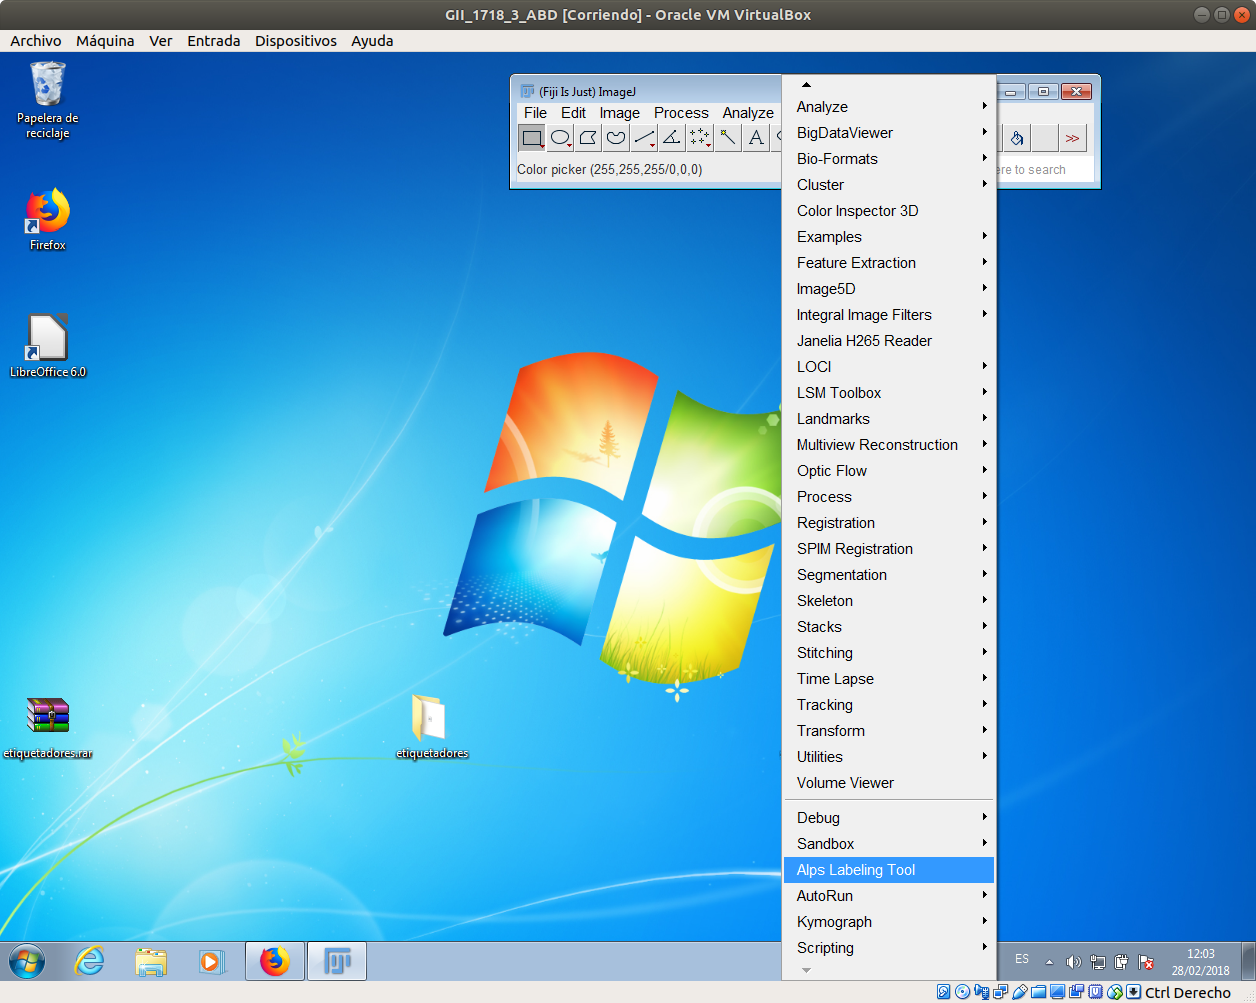
\includegraphics[width=0.7\linewidth]{img/AlpsLTPlugin}
		\caption{Plugin Alps Labeling Tool}
		\label{fig:alpsltplugin}
	\end{figure}
	Esta barra de trabajo contiene 6 funcionalidades básicas:
	\begin{enumerate}
		\item \textbf{OPEN IMAGES \& LABELS.} Con esta opción del menú vamos a seleccionar la imagen con la que vamos a trabajar. Lo ideal es seleccionar la primera imagen del directorio donde tengamos las imágenes para poder trabajar de forma ordenada, rápida y más segura.
		\item \textbf{SAVE LABELS.} Una vez hayamos realizado el etiquetado sobre la imagen podremos guardar en un .txt con las coordenadas de cada etiqueta de la imagen.
		\item \textbf{SAVE LABELS \& CLOSE.}Cuando ya hemos hecho el etiquetado sobre la imagen, si seleccionamos esta opción, nos permitirá guardar los datos de las etiquetas de la imagen y después cierra dicha imagen.
		\item \textbf{SAVE LABELS \& IMAGE.} Con esta opción podemos guardar la imagen con la información en otro directorio.
		\item \textbf{Flecha amarilla.} Nos carga la siguiente imagen del directorio.
		\item \textbf{Información.} Es la ayuda de la aplicación.
		
	\end{enumerate}
	
	\item \textbf{Cargar Imágenes.} Para poder trabajar etiquetando las imágenes, antes tenemos que cargarlas para visualizarlas. Para ello seleccionamos la opción \textit{OPEN IMAGES \& LABELS.}. Nos va a permitir navegar entre directorios para seleccionar finalmente qué imagen queremos etiquetar.
	Una vez esté la imagen abierta, la vista será similar a la mostrada en la imagen \ref{fig:etiquetado0}.
	\begin{figure}
		\centering
		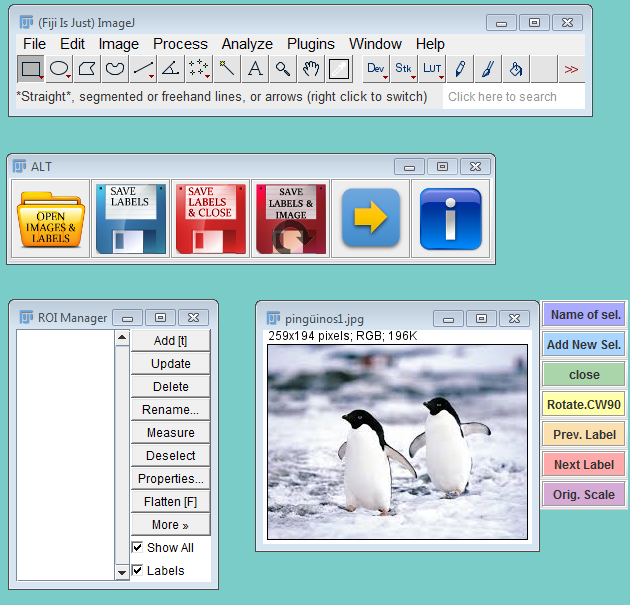
\includegraphics[width=0.7\linewidth]{img/etiquetado0}
		\caption{Estado de la aplicación antes del etiquetado}
		\label{fig:etiquetado0}
	\end{figure}
	
	\item \textbf{Etiquetado.} Para realizar el etiquetado dentro de una imagen que previamente hemos cargado tenemos que dibujar un rectángulo con el puntero sobre dicha imagen.
	Vamos a ponerle nombre a la etiqueta que hemos dibujado, para ello, una vez dibujado el rectángulo, pulsamos \textit{Add New Sel} en la columna de botones que hay a la derecha de la imagen. Ver imagen \ref{fig:etiquetapingu}.
	\begin{figure}
		\centering
		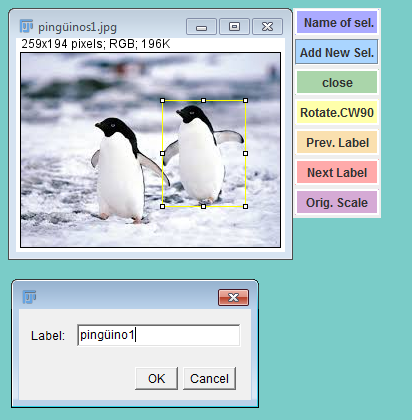
\includegraphics[width=0.7\linewidth]{img/etiquetapingu}
		\caption{Nombrar una etiqueta}
		\label{fig:etiquetapingu}
	\end{figure}
	
	En el caso de que después necesitásemos saber el nombre de la etiqueta que hemos puesto, manteniendo la etiqueta seleccionada, le damos a \textit{Name of sel} y nos dirá el nombre.
	\item \textbf{Guardar imágenes y etiquetas.} Una vez lo tenemos todo etiquetado dentro de la imagen tenemos que guardar la información generada por el etiquetado.
	Para llevar esto a cabo tenemos tres opciones: Guardar sólo las etiquetas y continuar etiquetando, guardar etiquetas y salir o guardar etiquetas e imágenes.
	Preferiblemente vamos a darle a la opción (en el menú ALT) de guardar etiquetas e imágenes y guardar todas las etiquetas en la misma carpeta de resultados para trabajar mejor con ellas.
	\item \textbf{Generar datos.}
	
\end{itemize}
\subsubsection{Recomendaciones}
He subido una máquina virtual a One Drive para que no sea necesario hacer ninguna instalación. Se puede acceder a la descarga desde \href{https://universidaddeburgos-my.sharepoint.com/:f:/g/personal/mmb0093_alu_ubu_es/EmokrIxFowNKvCanhqclkqkB90ruM7w-TPeXQS1MQQNmCQ?e=HMXXW4}{aquí}.
	
	
	\bibliographystyle{plain}
	\bibliography{bibliografiaAnexos}
	
\end{document}